%% @Author: Ines Abdeljaoued Tej
%  @Date:   2018-02
%% @Class:  Graduation Project, ESSAI - Carthage University, Tunisia.

\documentclass[a4paper, oneside]{report}

\usepackage[nottoc]{tocbibind}
\addcontentsline{toc}{section}{References}

\providecommand{\keywords}[1]{\textbf{\textit{Keywords---}} #1}

\usepackage{etoolbox}
%\makeatletter
%\patchcmd{\thebibliography}{%
%  \chapter*{\bibname}\@mkboth{\MakeUppercase\bibname}%{\MakeUppercase\bibname}}{%
%  \section{References}}{}{}
%\makeatother

\usepackage[utf8]{inputenc}
\usepackage[english]{babel}

\usepackage[nottoc]{tocbibind}

\textwidth 18cm
\textheight 24cm
\topmargin -0.5cm
\oddsidemargin -1cm

% set font encoding for PDFLaTeX or XeLaTeX
\usepackage{ifxetex}
\ifxetex
  \usepackage{fontspec}
\else
  \usepackage[T1]{fontenc}
  \usepackage[utf8]{inputenc}
  \usepackage{lmodern}
\fi


% Enable SageTeX to run SageMath code right inside this LaTeX file.
% documentation: http://mirrors.ctan.org/macros/latex/contrib/sagetex/sagetexpackage.pdf
%\usepackage{sagetex}


\newcommand{\reportTitle} {%
  \textsc{Graduation Project Report}
  %\textsc{Projet de Fin d'\'etudes}
}

\newcommand{\reportAuthor} {%
  FirstName \textsc{LastName}%
}

\newcommand{\reportSubject} {%
  My very attractive \\ Title%
}

\newcommand{\dateSoutenance} {%
  12/06/2018%
}

\newcommand{\studyDepartment} {%
  Entreprise d'accueil %Statistique
}

\newcommand{\ESSAI} {%
  Higher School of Statistics and Information Analysis
  %Ecole Sup\'erieure de la Statistique et de l'Analyse de l'Information
}

%\newcommand{\codePFE} {% Reference
%  Code PFE%
%}

\newcommand{\juryPresident} {%
  Mr Ben Foulen \textsc{Foulenia}%
}
\newcommand{\juryPresidentDesc} {%
  President%
}

\newcommand{\juryMemberOne} {%
  Ms Ben Foulena \textsc{Foulen}%
}
\newcommand{\juryMemberOneDesc} {%
  Supervisor %Mentor
}

\newcommand{\juryMemberTwo} {%
  Mr Ben Foulen \textsc{Fouleni}%
}
\newcommand{\juryMemberTwoDesc} {%
  Reviewer% Examiner, Reporter
}

\newcommand{\specialcell}[1]{%
  \begin{tabularx}{\textwidth}{@{}X@{}}#1\end{tabularx}%
}

%%%%%%%%%%%%%%%%%%%%%%%%%%%%%%%%%%%%%%%%%%%%%%%%%%%%%%%
% Add your own commands here
%%%%%%%%%%%%%%%%%%%%%%%%%%%%%%%%%%%%%%%%%%%%%%%%%%%%%%%
\newcommand{\MyCommand} {%
  Does nothing really%
}


% used in maketitle
\title{\reportSubject}
\author{\reportAuthor}

% Enable SageTeX to run SageMath code right inside this LaTeX file.
% documentation: http://mirrors.ctan.org/macros/latex/contrib/sagetex/sagetexpackage.pdf
%\usepackage{sagetex}

%\hypersetup{
%  pdftitle={\reportTitle~-~\reportSubject},%
%  pdfauthor={\reportAuthor},%
%  pdfsubject={\reportSubject},%
%  pdfkeywords={report} {internship} {pfe} {enis}
%}

\usepackage{graphics}
\usepackage{graphicx}

\begin{document}

\thispagestyle{empty}
\begin{titlepage}
\begin{center}


%%%%%%%%%%%%%%%%%%%%%%%%%%%%%%%%%%%%%%%%%%%%%%%
% THE HEADER
%%%%%%%%%%%%%%%%%%%%%%%%%%%%%%%%%%%%%%%%%%%%%%%

\includegraphics[width=2cm, height=1.5cm]{embleme.jpg}\\

{%
  \fontsize{9pt}{9pt}\selectfont%
  \begin{tabular}{c}
    Tunisian Republic\\
    Ministry of Higher Education and Scientific Research \\%
    Carthage University - \ESSAI{}  \\
    % Column 2
    %\studyDepartment \\
    % Engineering Education Computer Engineering and Applied Mathematics Discipline%
    % Cycle de Formation d'Ing\'enieurs en  Statistique et Analyse de l'Information%
    %Carthage University
  \end{tabular}
}

\vspace{10pt}

\includegraphics[width=4cm, height=2.5cm]{universite-carthage.jpg} \\

%%%%%%%%%%%%%%%%%%%%%%%%%%%%%%%%%%%%%%%%%%%%%%%
% THE PAGE CONTENT
%%%%%%%%%%%%%%%%%%%%%%%%%%%%%%%%%%%%%%%%%%%%%%%

\vspace{30pt} {%
  \renewcommand*{\familydefault}{\defaultFont}
  \fontsize{46pt}{46pt}\selectfont%
  % MEMOIRE\\%
  %\reportTitle{}%\\\textsc{Report}\\%
}

\vspace{30pt}
\textbf{\textit{Graduation Project Report submitted in partial fulfillment of}}\\
\textbf{\textit{the requirements for the degree of}}\\

\vspace{10pt}
Engineering Diploma in Statistics and Data Analysis\\


\includegraphics[width=2.5cm, height=2.5cm]{logo-essai.jpg}\\

\vspace{30pt}
\textbf{\textit{Submitted by}}\\
\vspace{10pt} {%
  \fontsize{18pt}{18pt}\selectfont%
  \textbf{\reportAuthor}\\
}%

\vspace{10pt} {%
  \renewcommand*{\familydefault}{\defaultFont}
  \fontsize{27pt}{27pt}\selectfont%
  \rule{0.5\textwidth}{.4pt}\\
  \vspace{10pt}
  \reportSubject{}\\%
  \vspace{10pt}
  \rule{0.5\textwidth}{.4pt}
}

\vspace{10pt}
Defended on~\dateSoutenance~ in front of the committee composed of:\\
%Soutenu le \dateSoutenance, devant la commission d'examen:\\
\vspace{20pt}
\begin{tabular}{p{0.3\linewidth} p{0.15\linewidth}}
  \juryPresident{} & \juryPresidentDesc{}\\
  \juryMemberOne{} & \juryMemberOneDesc{}\\
  \juryMemberTwo{} & \juryMemberTwoDesc{}\\
\end{tabular}

\vfill

\vspace{30pt}%
\textbf{\textit{A Graduation Project made at}}\\

\vspace{10pt}
(\studyDepartment)\\

\end{center}
\end{titlepage}

%\begin{pfe-essai}
%%%%%%%%%%%%%%%%%%%%%%%%%%%%%%%%%%%%%%%%%%%%%%%%%%%%%%%
% Table des matières, figures, tableaux ; Glossaire
%%%%%%%%%%%%%%%%%%%%%%%%%%%%%%%%%%%%%%%%%%%%%%%%%%%%%%%

\tableofcontents
\addcontentsline{toc}{chapter}{\contentsname}
\cleardoublepage%

\listoffigures
\addcontentsline{toc}{chapter}{\listfigurename}
\cleardoublepage%

\listoftables
\addcontentsline{toc}{chapter}{\listtablename}
\cleardoublepage

%    \printacronyms[heading=chapter*, name=Acronyms]
    %\printacronyms[heading=chapter*, name=Notations]

    %\addcontentsline{toc}{chapter}{Acronyms}
    %\addcontentsline{toc}{chapter}{Glossaire ou Notations}
    \cleardoublepage%

    \sloppy

    \pagenumbering{arabic}% 1 2 3 4 5
%    \doublespacing{}% Double spacing between lines

    \addtocontents{toc}{\protect\setcounter{tocdepth}{2}}


% ###############################
% # HELP COMMANDS               #
% ###############################
%
% -1 \part{part}
%  0 \chapter{chapter}
%  1 \section{section}
%  2 \subsection{subsection}
%  3 \subsubsection{subsubsection}
%  4 \paragraph{paragraph}
%  5 \subparagraph{subparagraph}


%%%%%%%%%%%%%%%%%%%%%%%%%%%%%%%%%%%%%%%%%%%%%%%%%%%%%%%
% Dédicace et Remerciements
%%%%%%%%%%%%%%%%%%%%%%%%%%%%%%%%%%%%%%%%%%%%%%%%%%%%%%%

\chapter*{Dedication}
%\chapter*{D\'edicace}
%\addcontentsline{toc}{chapter}{Dedication}
\thispagestyle{empty}
%
%For all they have endured to satisfy all my needs and wishes

\begin{center}
  Put your dedication lines here ~\\
  And try to be expressive ;) ~\\


  Lorem ipsum dolor sit amet, consectetur adipisicing elit, sed do eiusmod ~\\
  tempor incididunt ut labore et dolore magna aliqua. Ut enim ad minim veniam, ~\\
  quis nostrud exercitation ullamco laboris nisi ut aliquip ex ea commodo ~\\
  consequat. Duis aute irure dolor in reprehenderit in voluptate velit esse ~\\
  cillum dolore eu fugiat nulla pariatur. Excepteur sint occaecat cupidatat non ~\\
  proident, sunt in culpa qui officia deserunt mollit anim id est laborum ~\\
\end{center}
%
%\nopagebreak{%
% And maybe a quote here
% \raggedright\hspace{5.75cm} To all of you,~\\
%\raggedright\hspace{7.75cm} I dedicate this work.
%  \raggedleft\normalfont\large\itshape{} \reportAuthor\par%
%}
%
%\cleardoublepage%

\chapter*{Thanks}
%\chapter*{Remerciements}
%\addcontentsline{toc}{chapter}{Thanks}
\thispagestyle{empty}

And put your thanks here. \\

Lorem ipsum dolor sit amet, consectetur adipisicing elit, sed do eiusmod
tempor incididunt ut labore et dolore magna aliqua. Ut enim ad minim veniam,
quis nostrud exercitation ullamco laboris nisi ut aliquip ex ea commodo
consequat. Duis aute irure dolor in reprehenderit in voluptate velit esse \cite{caillois1}
cillum dolore eu fugiat nulla pariatur. Excepteur sint occaecat cupidatat non
proident, sunt in culpa qui officia deserunt mollit anim id est laborum. Lorem ipsum dolor sit amet, consectetur adipisicing elit, sed do eiusmod
tempor incididunt ut labore et dolore magna aliqua. Ut enim ad minim veniam,
quis nostrud exercitation ullamco laboris nisi ut aliquip ex ea commodo
consequat. Duis aute irure dolor in reprehenderit in voluptate velit esse
cillum dolore eu fugiat nulla pariatur. Excepteur sint occaecat cupidatat non
proident, sunt in culpa qui officia deserunt mollit anim id est laborum.



%%%%%%%%%%%%%%%%%%%%%%%%%%%%%%%%%%%%%%%%%%%%%%%%%%%%%%%
% Divers chapitres
%%%%%%%%%%%%%%%%%%%%%%%%%%%%%%%%%%%%%%%%%%%%%%%%%%%%%%%


\chapter*{Introduction}
\label{chap:general_intorduction}
\markboth{\MakeUppercase{Introduction}}{}%
\addcontentsline{toc}{chapter}{Introduction}%

%Welcome to \Ac{ESSAI}. ~\\
%Again, welcome to \Ac{ESSAI}. ~\\
%Your introduction goes here. ~\\

Lorem ipsum dolor sit amet, consectetur adipisicing elit, sed do eiusmod
tempor incididunt ut labore \cite{jenkins2004} et dolore magna aliqua. Ut enim ad minim veniam,
quis nostrud exercitation ullamco laboris nisi ut aliquip ex ea commodo
consequat \cite{hui}. Duis aute irure dolor in reprehenderit in voluptate v.


Voici une référence à l'image de la figure \ref{fig:pictureTwo} page \pageref{fig:pictureTwo} et une autre vers la partie \ref{chapter2} page \pageref{chapter2}.
On peut citer un livre\, \cite{caillois1} et on précise les détails à la fin du rapport dans la partie références.
Voici une note\,\footnote{Texte de bas de page} de bas de page\footnote{J'ai bien dit bas de page}.


\begin{itemize}
  \item The individual entries are indicated with a black dot, a so-called bullet.
  \item The text in the entries may be of any length.
\end{itemize}

\chapter{Chapter One}%
\label{chap:chapterone}

%%%%%%%%%%%%%%%%%%%%%%%%%%%%
% SECTION                  %
%%%%%%%%%%%%%%%%%%%%%%%%%%%%
\section{Section One}
\label{chap:sectionone}

\subsection{Sub section One}

And your chapter one goes here \cite{web001,Nom2012}. \\
  Lorem ipsum dolor sit amet, consectetur adipisicing elit, sed do eiusmod
  tempor incididunt ut labore et dolore magna aliqua. Ut enim ad minim veniam, quis nostrud exercitation ullamco laboris nisi ut aliquip ex ea commodo consequat. Duis aute irure dolor in reprehenderit in voluptate velit esse
  cillum dolore eu fugiat nulla pariatur. Excepteur sint occaecat cupidatat non
  proident, sunt in culpa qui officia deserunt mollit anim id est laborum.

  \begin{figure}[h]%
    \center%
    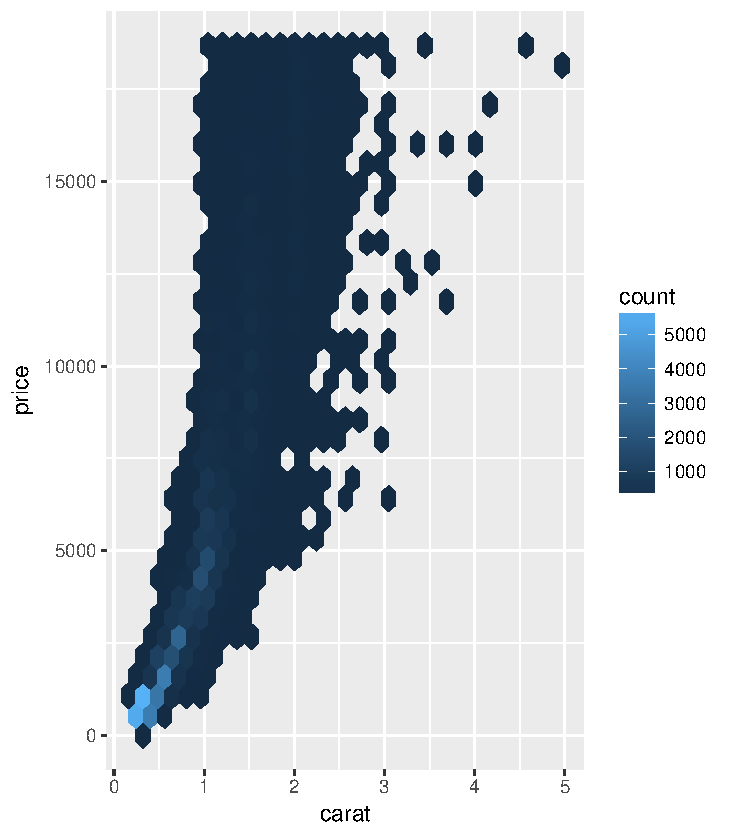
\includegraphics[width=0.3\textwidth]{diamonds.pdf}%
    \caption[This is a test image]{Test Image}\label{fig:test}%
  \end{figure}


\begin{table}
\begin{tabular}{cc}
A & B \\
C & D
\end{tabular}
\caption{Test Table}
\end{table}

 \subsection{Sub section Two}

  This is a second subsection\cite{gen1972}, \cite{schaeffer99}. ~\\
  Lorem ipsum dolor sit amet, consectetur adipisicing elit, sed do eiusmod
  tempor incididunt ut labore et dolore magna aliqua. Ut enim ad minim veniam,
  quis nostrud exercitation ullamco laboris nisi ut aliquip ex ea commodo
  consequat. Duis aute irure dolor in reprehenderit in voluptate velit esse
  cillum dolore eu fugiat nulla pariatur. Excepteur sint occaecat cupidatat non
  proident, sunt in culpa qui officia deserunt mollit anim id est laborum.

  \begin{description}\addtolength{\itemsep}{-0.35\baselineskip}%
    \item[\textbullet~\bfseries Menu Item] \hfill \\%
      Menu Description.~\\%
      {\textbf{Focus topics:~}\emph{Topic one, topic two, topic three, ...}}%
    %
    \item[\textbullet~\bfseries Menu Item] \hfill \\%
      Menu Description.~\\%
      {\textbf{Focus topics:~}\emph{Topic one, topic two, topic three, ...}}%
    %
    \item[\textbullet~\bfseries Menu Item] \hfill \\%
      Menu Description.~\\%
      {\textbf{Focus topics:~}\emph{Topic one, topic two, topic three, ...}}%
  \end{description}

  Also bullets such as:%
  \begin{itemize}\addtolength{\itemsep}{-0.35\baselineskip}%
    \item One%
    \item Two%
    \item Three%
    \item Four%
    \item \ldots%
  \end{itemize}%
  %
\subsection{powers series} \label{subsection}

\begin{equation} \label{eq:1}
\sum_{i=0}^{\infty} a_i x^i
\end{equation}

The equation \ref{eq:1} is a typical power series.

\chapter*{Autre chapitre}
\label{chapter2}
\markboth{\MakeUppercase{Autrechap}}{}%
\addcontentsline{toc}{chapter}{Autre Chapitre}%

\chapter*{Conclusion}
\label{chap:conclusion}
\markboth{\MakeUppercase{Conclusion}}{}%
\addcontentsline{toc}{chapter}{Conclusion}
  And a very interesting conclusion here\@. ~\\
  Lorem ipsum dolor sit amet, consectetur adipisicing elit, sed do eiusmod
  tempor incididunt ut labore et dolore magna aliqua. Ut enim ad minim veniam,
  quis nostrud exercitation ullamco laboris nisi ut aliquip ex ea commodo
  consequat.

\chapter*{Appendix}
\label{chap:appendix}
\markboth{\MakeUppercase{Appendix}}{}
\addcontentsline{toc}{chapter}{Appendix}

  An appendix if you need it. ~\\

  Lorem ipsum dolor sit amet, consectetur adipisicing elit, sed do eiusmod
  tempor incididunt ut labore et dolore magna aliqua. Ut enim ad minim veniam,
  quis nostrud exercitation ullamco laboris nisi ut aliquip ex ea commodo.


\bibliographystyle{apalike}
\bibliography{Biblio}

\begin{abstract}

Put here an absract for the report; \\

\keywords{Insert 5 keywords}
\end{abstract}

\end{document}